\documentclass[aspectratio=169]{beamer}              % only frames

% for themes, etc.
\mode<presentation>
\usetheme{Madrid} 
\usecolortheme{crane}

%\usepackage{times}  % fonts are up to you
% The usual suspects
\usepackage{multirow, booktabs, dcolumn, color, graphicx} % Tables\usepackage{graphicx}
\usepackage{amsmath,amssymb,amsthm}
% Strikethrough text
\usepackage{soul}
% Adjust box to fit tabulars
\usepackage{adjustbox}
% Embed video
\usepackage{media9}
% For notes
\usepackage{pgfpages}
\setbeameroption{hide notes} % Only slides
%\setbeameroption{show only notes} % Only notes
%\setbeameroption{show notes on second screen=right} % Both
% Use colors by name
\usepackage{xcolor}
% EMBEDDING VIDEO IS POSSIBLE WITH PDFPC USE PDF PC to present
\usepackage{multimedia}



% The table highlighting for hypothesis discussion.
\usepackage[beamer,customcolors]{hf-tikz}
\usetikzlibrary{calc}

% To use background images
\newenvironment{colorframe}[2][]{%
\setbeamercolor{background canvas}{bg=#1}
\begin{frame}\color{white}}
{\end{frame}}


% To set the hypothesis highlighting boxes red.
\tikzset{hl/.style={
    set fill color=red!80!black!40,
    set border color=red!80!black,
  },
}

% Set Graphics folder
\graphicspath{{./figures/}}


% these will be used later in the title page
\title{Threatlandscape}
\subtitle{Threat Actors}
\author{Irfan Kanat}
\institute[CBS]{{Department of Digitization}\\ Copenhagen Business School}
%\date{\today}



\begin{document}

% this prints title, author etc. info from above
\begin{frame}

	\titlepage


	\vfill
	{\tiny \centering This work is licensed under a \href{http://creativecommons.org/licenses/by/4.0/}{Creative Commons Attribution 4.0 International License}.}

\end{frame}

\note{In this presentation we focus on threat actors.}


\begin{frame}
	\frametitle{Its on the News}

	    \begin{columns}
			\begin{column}{0.5\textwidth}
	
				
\includegraphics[width = \textwidth, height = .85\textheight, keepaspectratio]{figures/BBC.jpg}
		
			\end{column}
	
			\begin{column}{0.5\textwidth}
	
				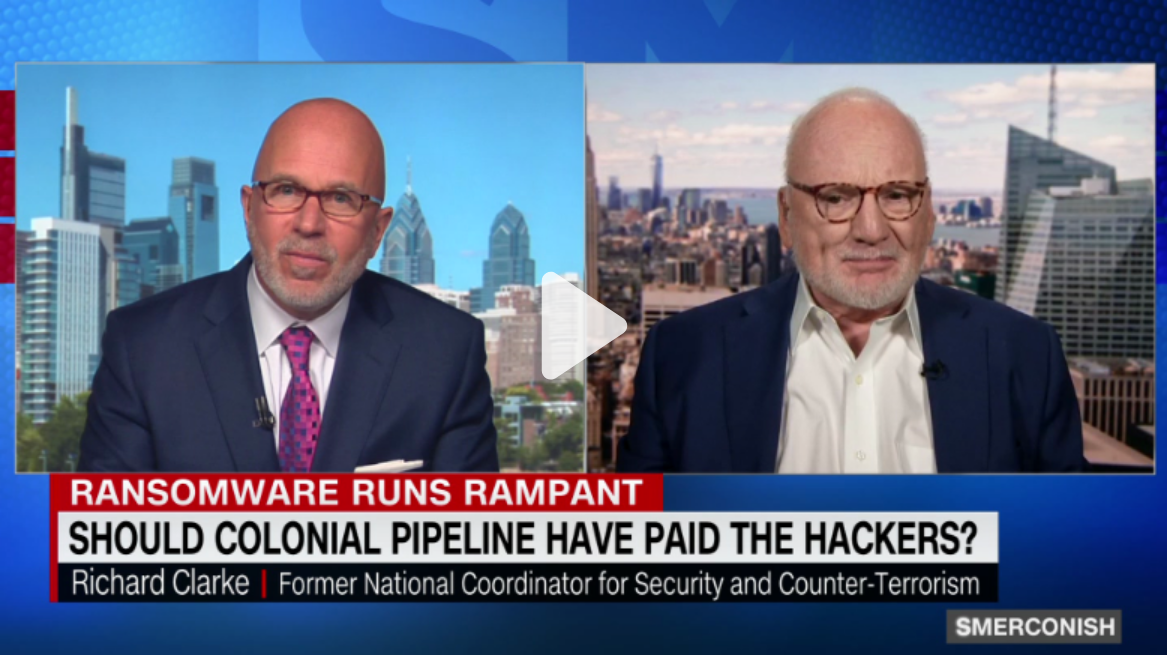
\includegraphics[width = \textwidth, height = .85\textheight, keepaspectratio]{figures/CNNColonialPipeline.png}
	
			\end{column}
	
		\end{columns}

\end{frame}

\note{Cybersecurity is in the news. You hear about ransomware, advanced persistent threats, hacks, vulnerabilities, 0days and more... But what do these words mean? That is what we will learn about today. In this video we will focus on different threat actors.}


\begin{frame}
	\frametitle{Big Question: Who is Who?}
    
    \begin{itemize}
    	\item Who all are out there?
    	\item What do they want?
    \end{itemize}

\end{frame}

\note{In this video we will learn about different threat actors. Who is behind the cyber threats? What do they want?}


\begin{frame}
	\frametitle{Know Your Threat Actors}
    
	\begin{columns}
		\begin{column}{0.5\textwidth}

		\begin{itemize}
			\item Organized Crime
			\item Hacktivist
			\item Insiders
			\item State Actors
		\end{itemize}
	
		\end{column}

		\begin{column}{0.5\textwidth}

			
\includegraphics[width = \textwidth, height = .85\textheight, keepaspectratio]{figures/Enemy.jpeg}

		\end{column}

	\end{columns}


\end{frame}

\note{In 2021 Organized crime made up over 80\% of data breaches. The rest of the breaches were the work of unaffiliated hackers, insiders and state sponsored groups.


\tiny{Source: Verizon DBIR 2021}}

\begin{frame}
\frametitle{Organized Crime}

	\movie{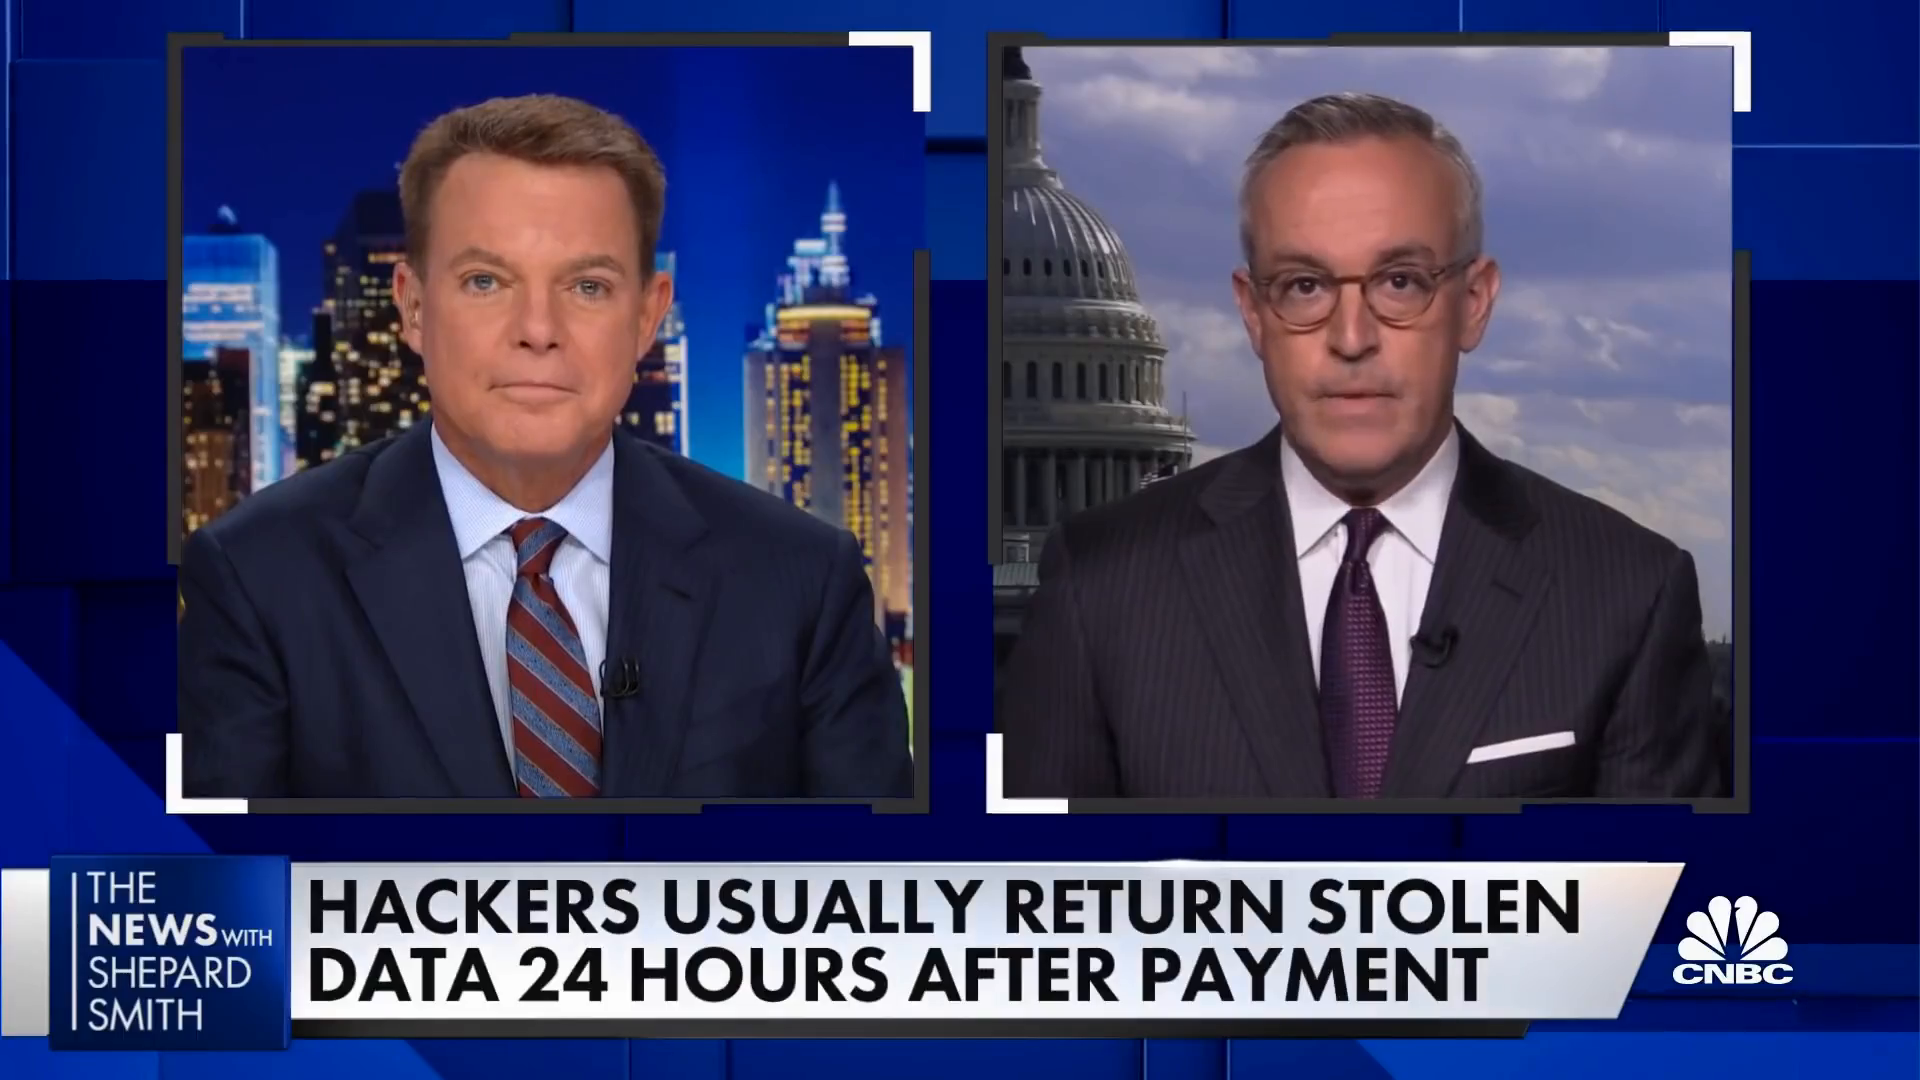
\includegraphics[width = \textwidth]{figures/WhereRansomGoes.png}}{figures/WhereRansomGoes.mp4}

\end{frame}

\note{No we don't mean mafia of course. Organized in the sense, they operate in an organized fashion. Have shifts, regular working hours, reporting structure. Cybercrime is a job.

Organized crime groups are motivated by financial gains. 

The increasing access to financial resources allows them to purchase more sophisticated hacking tools on the dark net. There is also some transitivity between some nation state groups and organized crime groups. These factors lead to blurring of the lines when it comes to the sophistication of these groups.

Their most recent exploits have centered around ransomware.}


\begin{frame}
	\frametitle{Hacktivist}
    
    \movie{
\includegraphics[width = \textwidth]{figures/Anonymous.png}}{figures/Anonymous.mp4}

\end{frame}

\note{Around 2010-2014 Hacktivism used to be a bigger problem. Non-affiliated, or loosely affiliated groups of hackers came together to further their political goals.

Since their goals are political their actions are a bit harder to predict than organized crime groups.

Although, Hacktivists hey day seems to have passed, there is still a steady stream of hacks originating from these groups. In 2021 Bellarusan hacktivists have hacked into the rail system of Bellarus, disrupting Russian weapons shipments to Ukraine border.
}

\begin{frame}
	\frametitle{Insiders}
    
    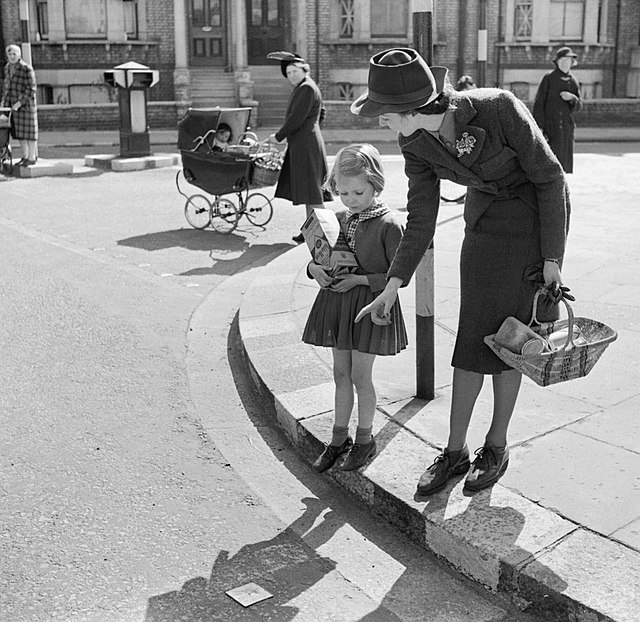
\includegraphics[width = \textwidth, height = .85\textheight, keepaspectratio]{figures/mom.jpeg}

\end{frame}

\note{Insiders are people who already have some legitimate access. Insiders can inflict harm on information assets through either ignorance, or malice. In case of malice, the motivation is often financial, or revenge.

A secretary sending PII over e-mail is a data breach of the error variety.

A system admin deleting contents of a server is malicious action.

Even if you have no administrative control, you are at threat from insiders in your household. That is why you use private browsing, and don't save passwords in your browser.
}


\begin{frame}
	\frametitle{State Actors}
    
	    \begin{columns}
			\begin{column}{0.5\textwidth}
	
				Espionage \vspace{1em}

				Sabotage \vspace{1em}

				And in one case simple theft...
		
			\end{column}
	
			\begin{column}{0.5\textwidth}
	
				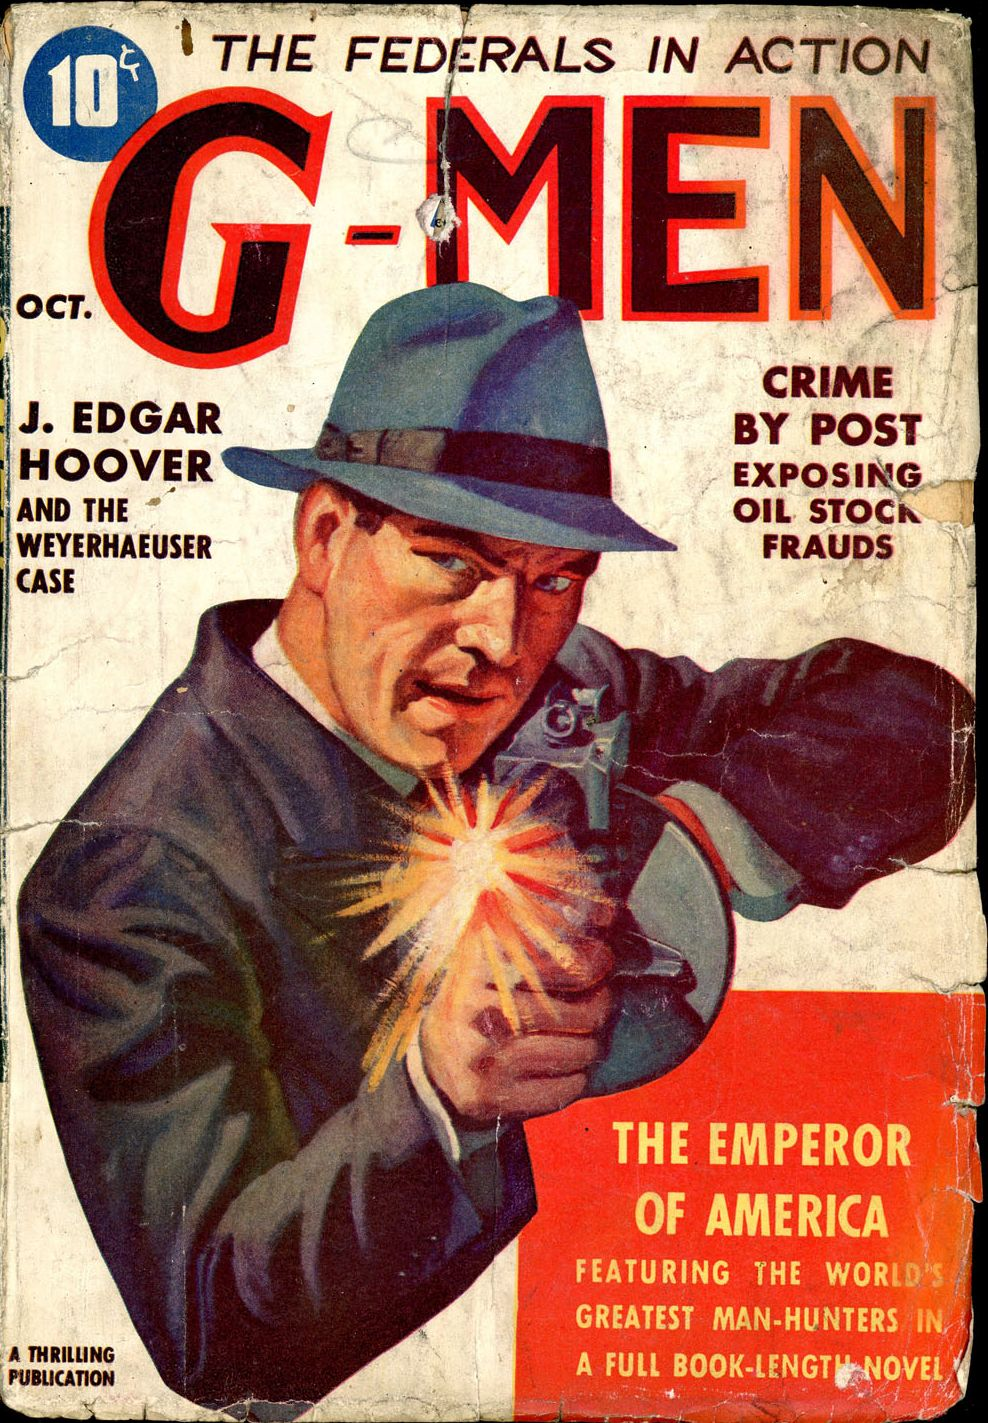
\includegraphics[width = \textwidth, height = .85\textheight, keepaspectratio]{figures/G-MEN.jpg}
	
			\end{column}
	
		\end{columns}

\end{frame}

\note{States employ well funded, well organized groups for strategic advantage. These groups often are the most sophisticated threats in the field. They have access to vast throves of vulnerabilities and exploits and they plan their intrusions with extreme care. Since they are motivated to see their actions through, they just persist in gaining access. Because of all these factors, they are often referred to as Advanced Persistent Threats.

Since their motivations are to gain strategic advantage for their states, they rarely are motivated by financial returns (North Korea is the sole exception). Mostly these groups are conducting espionage and sabotage actions.

Due to their competence and clandestine nature of their activities we know relatively little about their operations. What we glimpse is amazing to say the least. The most well known cases of State Actor actions were stuxnet, and notpetya.
}

\begin{frame}
	\frametitle{Threat Models}

    
	\centering


\adjustbox{max height=\dimexpr\textheight-5.5cm\relax,
           max width=\textwidth}{
\begin{tabular}{llll}
\textbf{Threat} &
  \begin{tabular}[c]{@{}l@{}}Ex-girlfriend/boyfriend breaking \\ into your email account and publicly\\  releasing your correspondence with\\  the My Little Pony fan club\end{tabular} &
  \begin{tabular}[c]{@{}l@{}}Organized criminals breaking\\  into your email account and \\ sending spam using your identity\end{tabular} &
  \begin{tabular}[c]{@{}l@{}}The Mossad doing Mossad\\ things with your email account\end{tabular} \\
\textbf{Solution} &
  Strong passwords &
  \begin{tabular}[c]{@{}l@{}}Strong passwords + common sense\\ (don’t click on unsolicited herbal \\ Viagra ads that result in keyloggers\\ and sorrow)\end{tabular} &
  \begin{tabular}[c]{@{}l@{}}Magical amulets?\\ \\ Fake your own death, move into a \\ submarine?\\ \\ YOU’RE STILL GONNA BE \\ MOSSAD’ED UPON\end{tabular}
	\end{tabular}}
		
    
\end{frame}

\note{Appropriate response is relative. Example here is from James Mickens. As he puts it so nicely: ``If Mossad wants to do Mossady things to you, you will get Mossadded upon.''

}

\end{document}
